A pesquisa e o desenvolvimento (P\&D) tem como propósito fomentar o avanço
tecnológico e novas maneiras de desenvolver tipos específicos de conhecimento
no país. O desenvolvimento do robô EMMA, no âmbito P\&D é um exemplo de como a
parceria entre agências do governo e uni- versidades federais podem colaborar
para a capacitação tecnológica e o desenvolvimento de novas tecnologias.
Especificamente na área de robótica, o projeto EMMA mostra como a otimização e
automação de diversos processos de trabalho pode contribuir na indústria
energética. Em termos acadêmicos, esta linha de projetos já originou %TODO
dissertações de mestrado no Programa de Engenharia Elétrica (PEE), Universidade
Federal do Rio de Janeiro (UFRJ), abordando os seguintes tópicos:

%TODO Julia e Estevao - Propostas

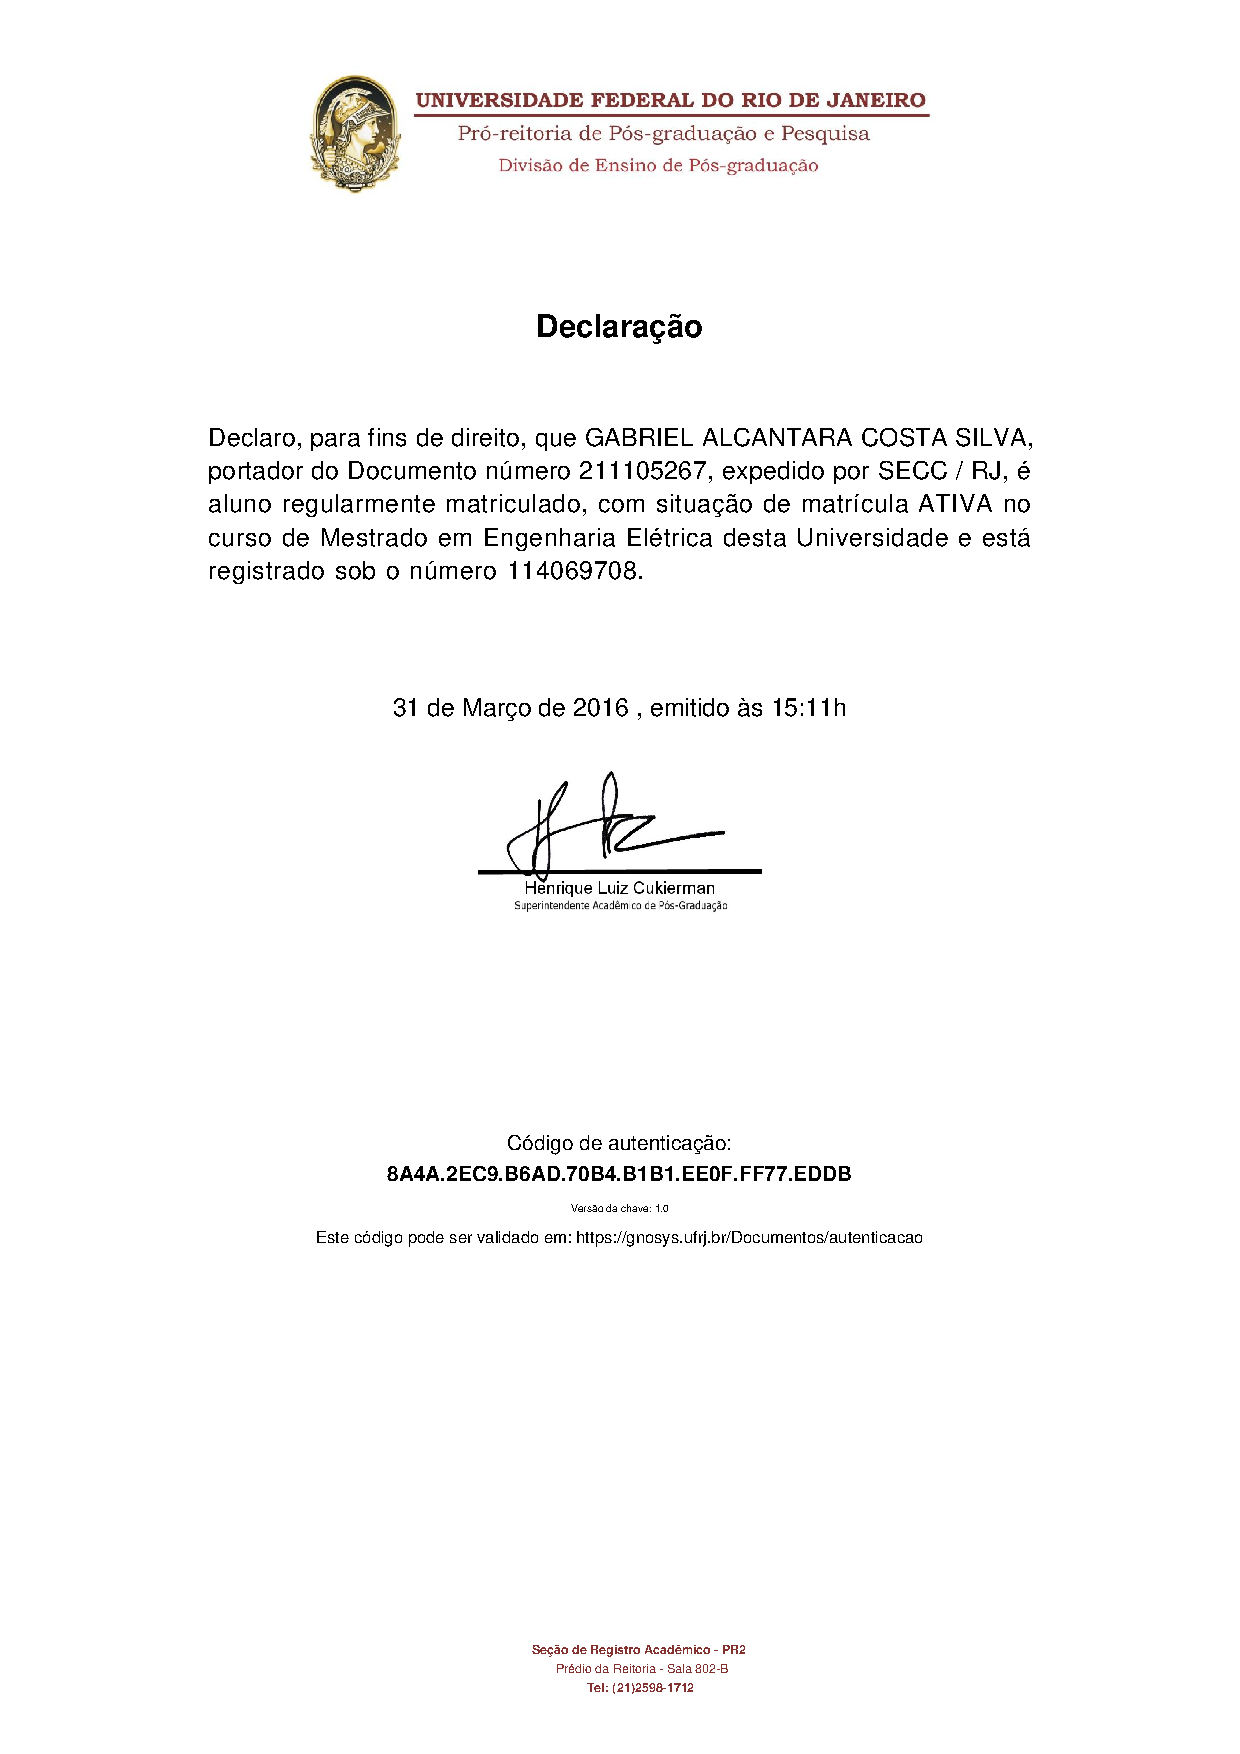
\includepdf{pdfs/mestrado_gabriel}
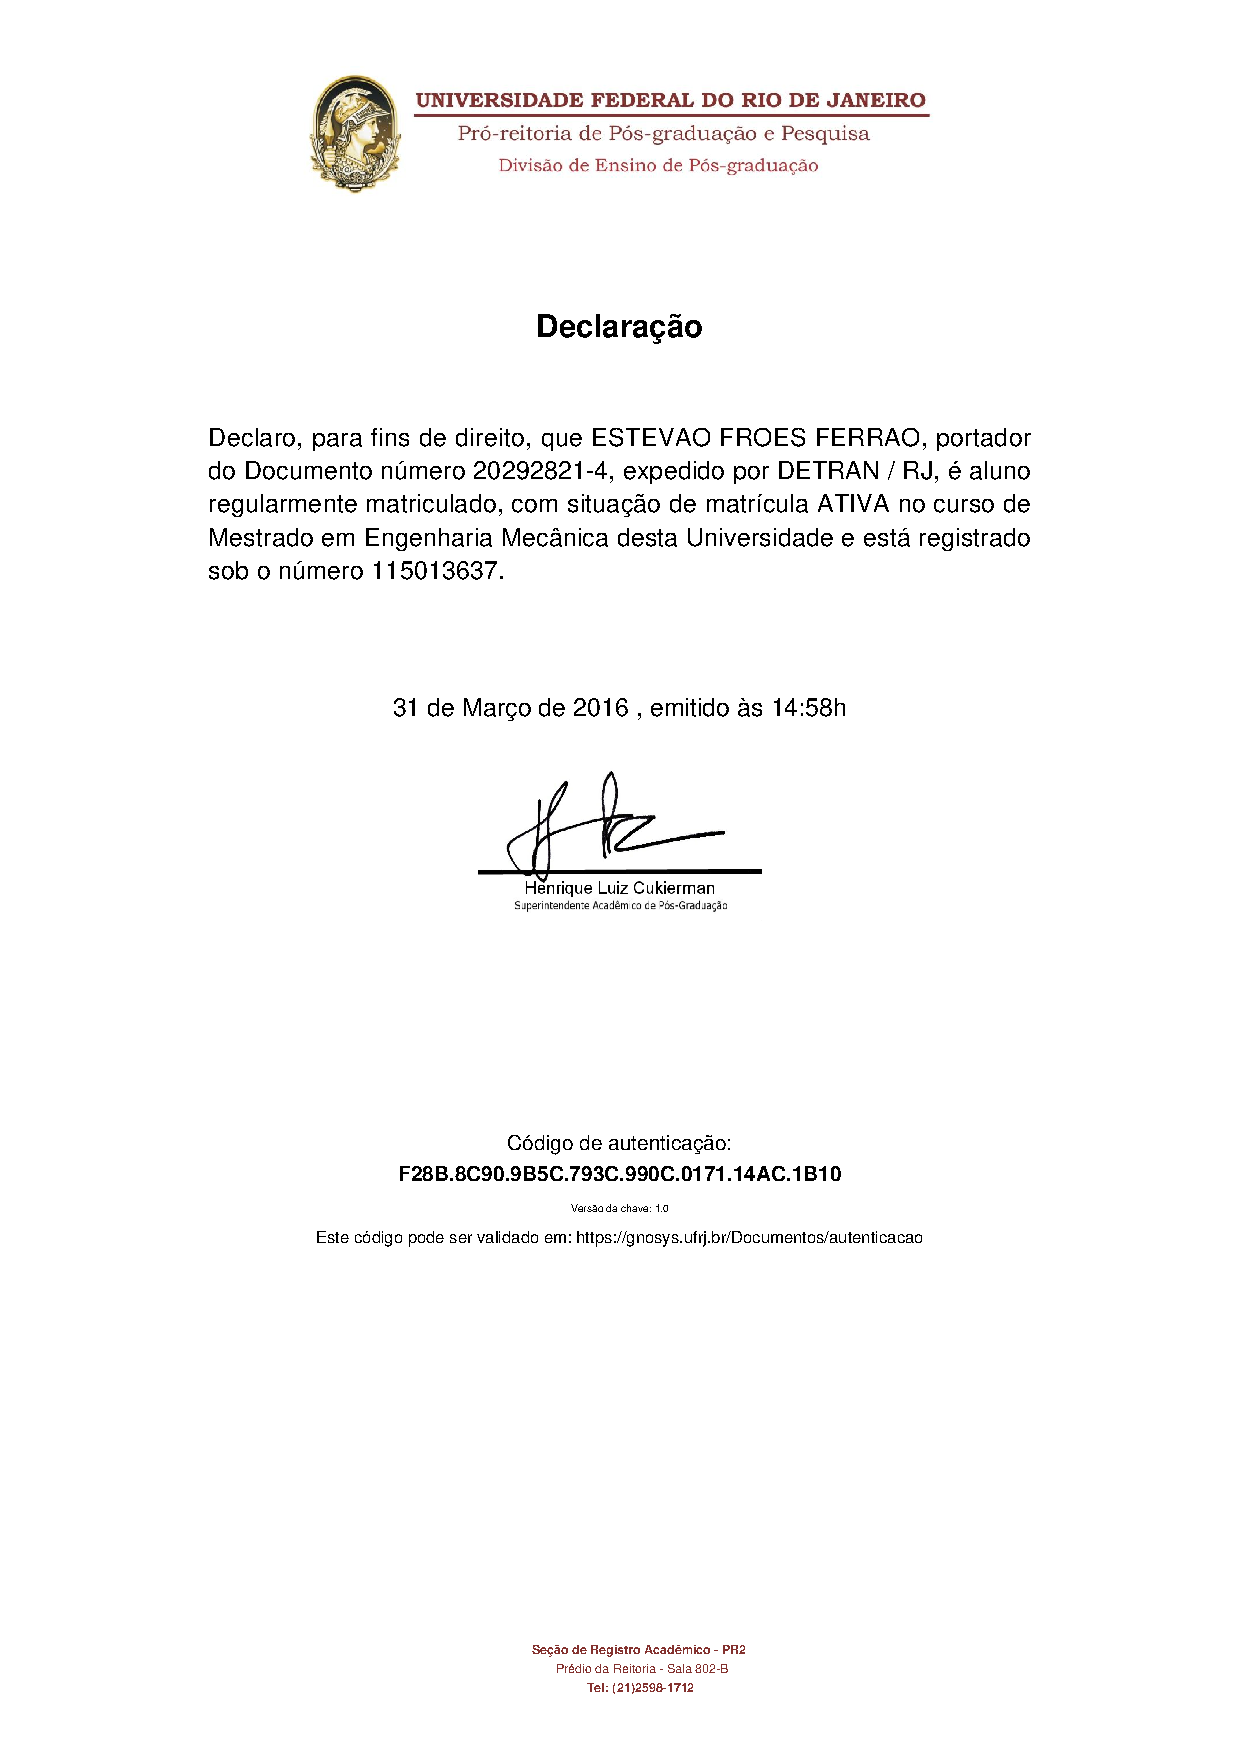
\includepdf{pdfs/mestrado_estevao}
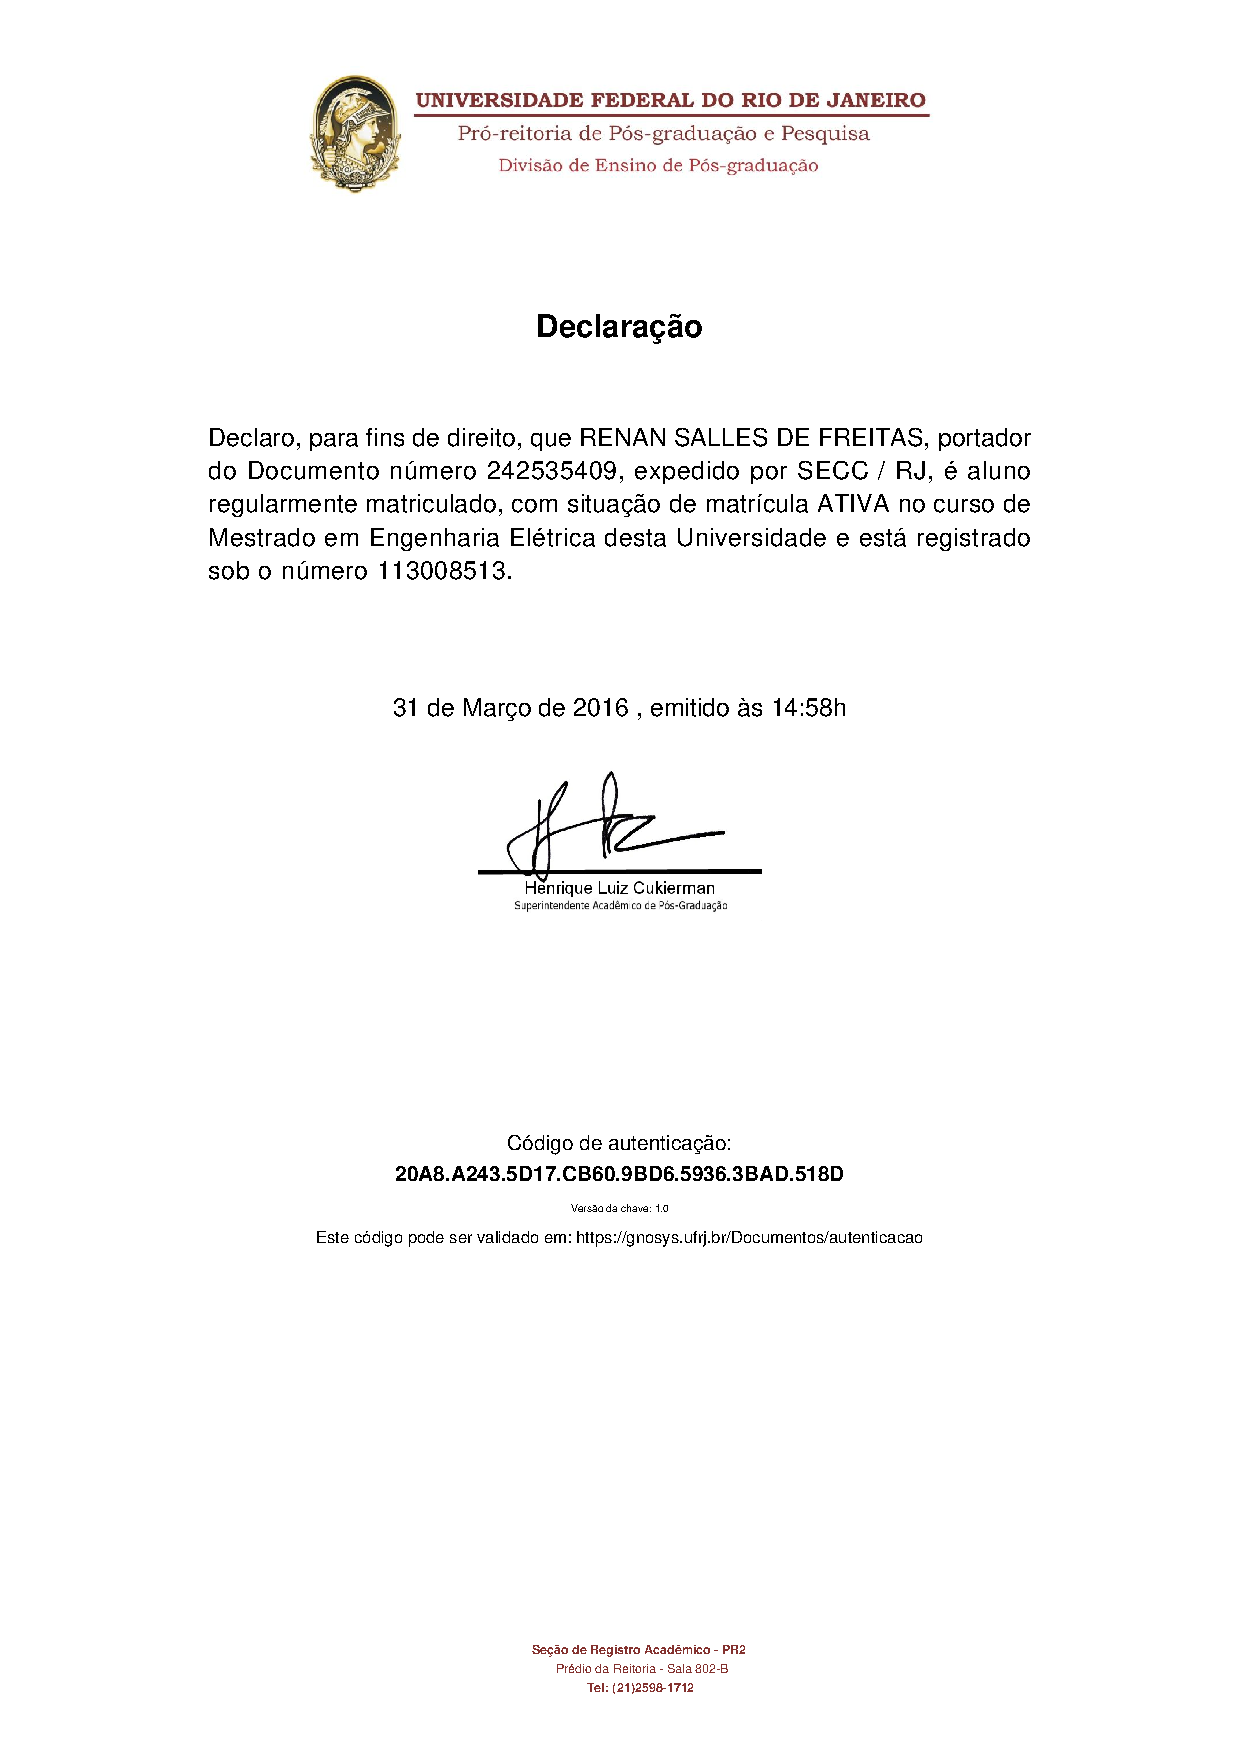
\includepdf{pdfs/mestrado_renan}
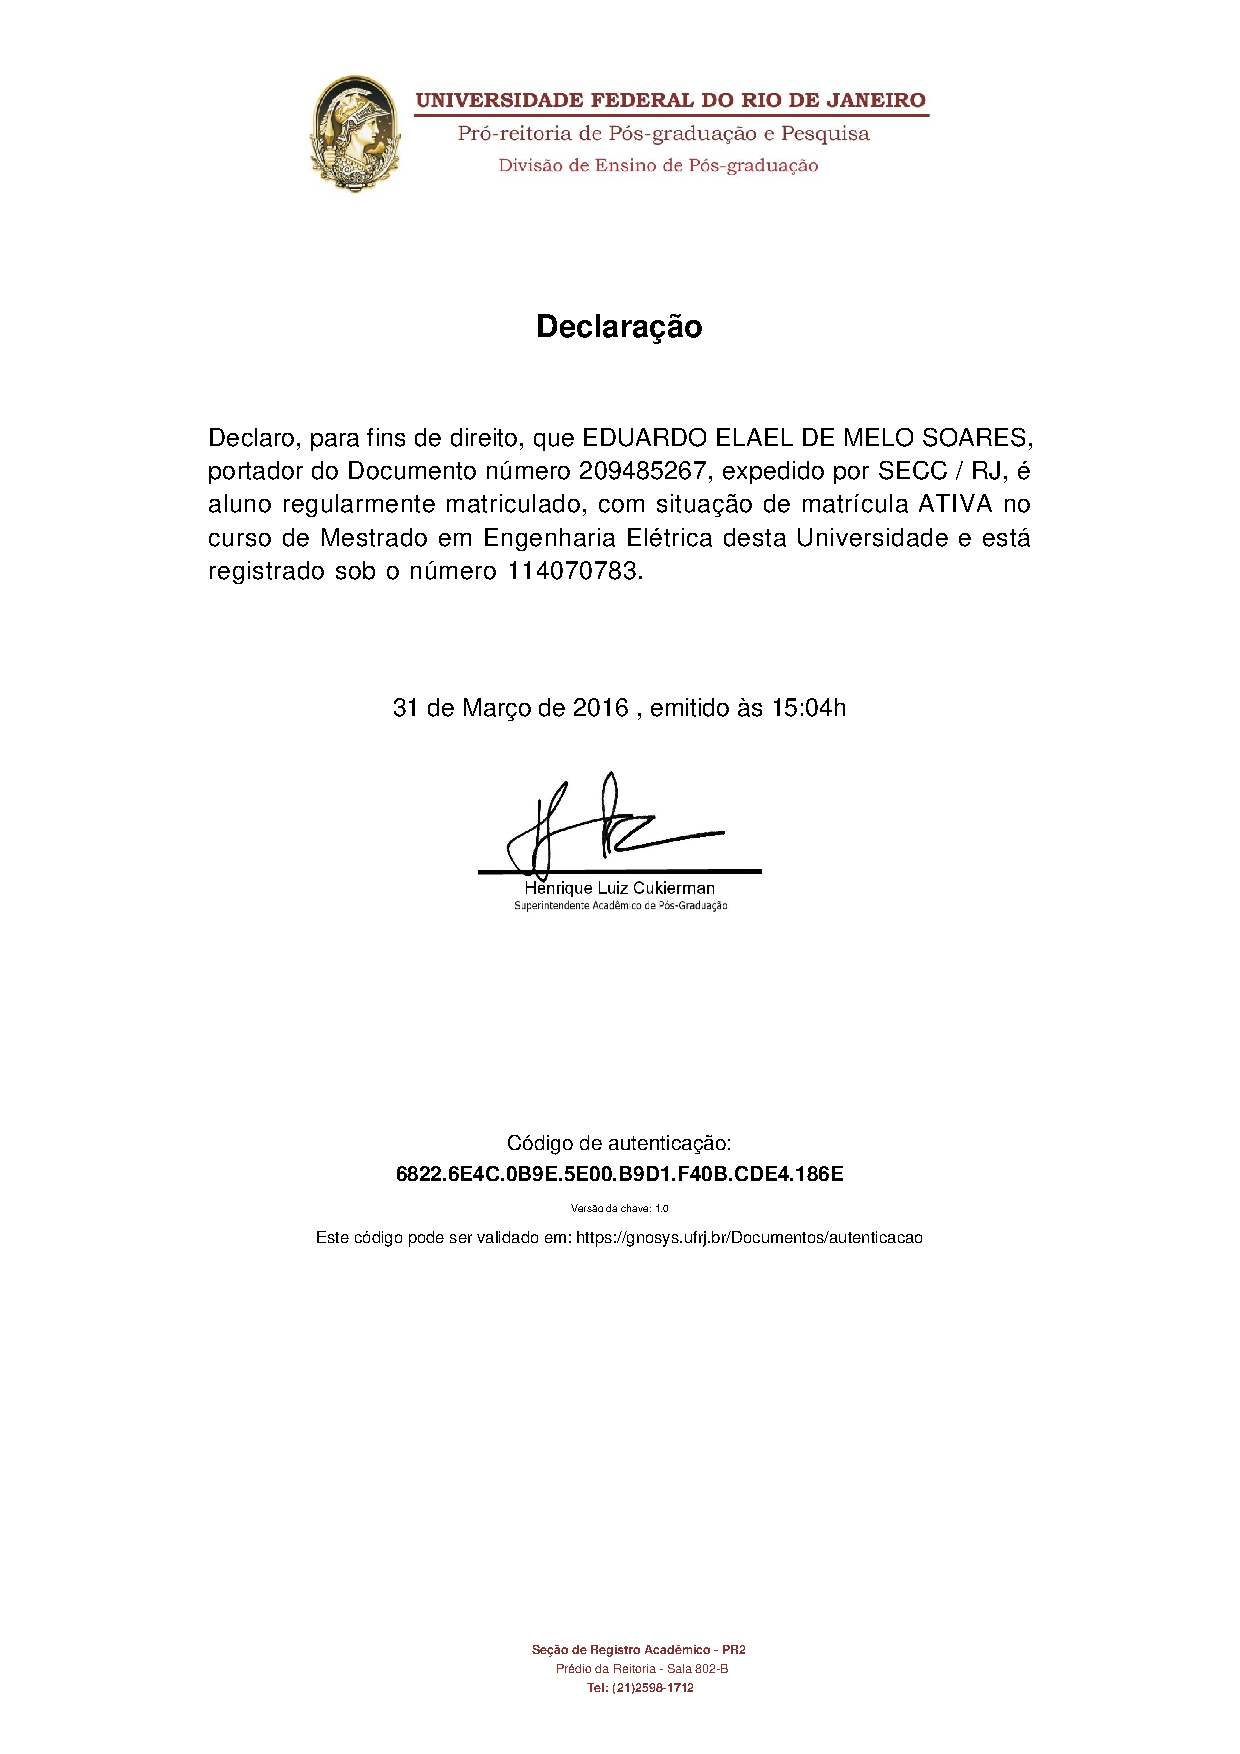
\includepdf{pdfs/mestrado_elael}